\chapter{システムコール呼び出し履歴を用いた検知手法による評価実験}
本研究で実装した検知システムにおける定常的な動作負荷の計測を行い,IoTデバイスが本来の動作を阻害しないことを評価する.DDoS攻撃を行うマルウェアを用いて検知精度の評価を行い,システムコール呼び出し履歴による検知手法でマルウェアが検出できることを確認した.

\section{システムコール呼び出し履歴を用いた検知手法による定常的な動作負荷の評価}

IoTデバイスにマルウェアが動作していない状況下において,提案した検知システムによるマルウェア探索動作によってIoTデバイス本来の動作が阻害されていないことを評価するために,3.4節で述べたように,LinuxOSを対象とする既存のアンチウィルスソフトであるClam AVを動作させた状態のCPU,メモリの使用率を基準値とし,提案した検知システムによってMiraiが動作していない状況での,CPU,メモリの使用率についてsarコマンドを用いて1分間計測を行った.
sarコマンドを用いて得たCPU,メモリの使用率について,Clam AVと比較を行った結果が図\ref{fig:strace_cpu},\ref{fig:strace_mem}になる.ClamAVを動作させた状態のIoTデバイスのCPU使用率,メモリ使用率の値は3.4節で計測したデータを用いた.
Clam AntiVirusを利用した場合には,平均CPU使用率が24.27\%,メモリ使用率は7.92\%であり.提案した検知手法では,平均CPU使用率が0.57\%,メモリ使用率が4.08\%となった.メモリ使用率は比較対象のClam AntiVirusと提案した検知手法では97.6\%減,CPU使用率は,Clam AntiVirusに対して提案した検知手法は48.4\%減となった.


\clearpage
\begin{figure}[h]
    \centering
       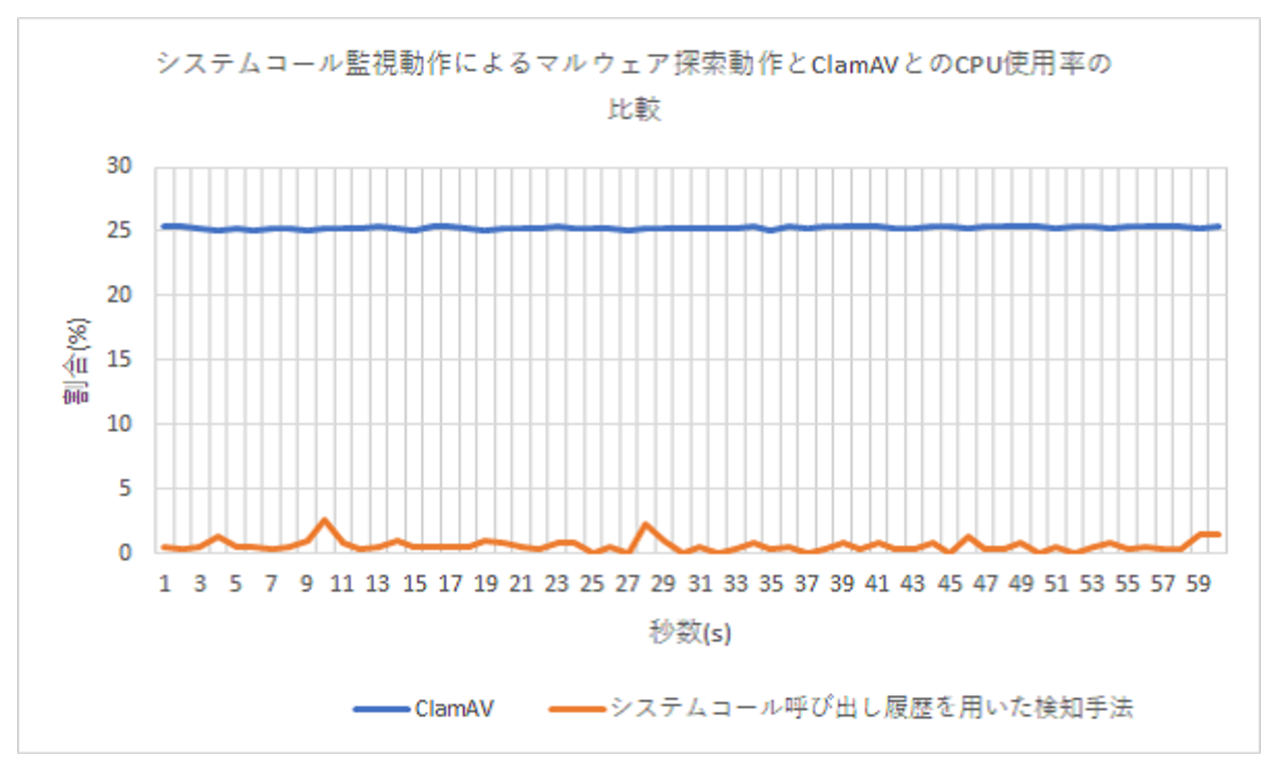
\includegraphics[width=110mm]{figures/strace_cpu.eps}
    \caption{システムコール呼び出し履歴によるマルウェア探索動作とClamAVとのCPU使用率の比較}
        \label{fig:strace_cpu}
\end{figure}
  
\begin{figure}[h]
        \centering
           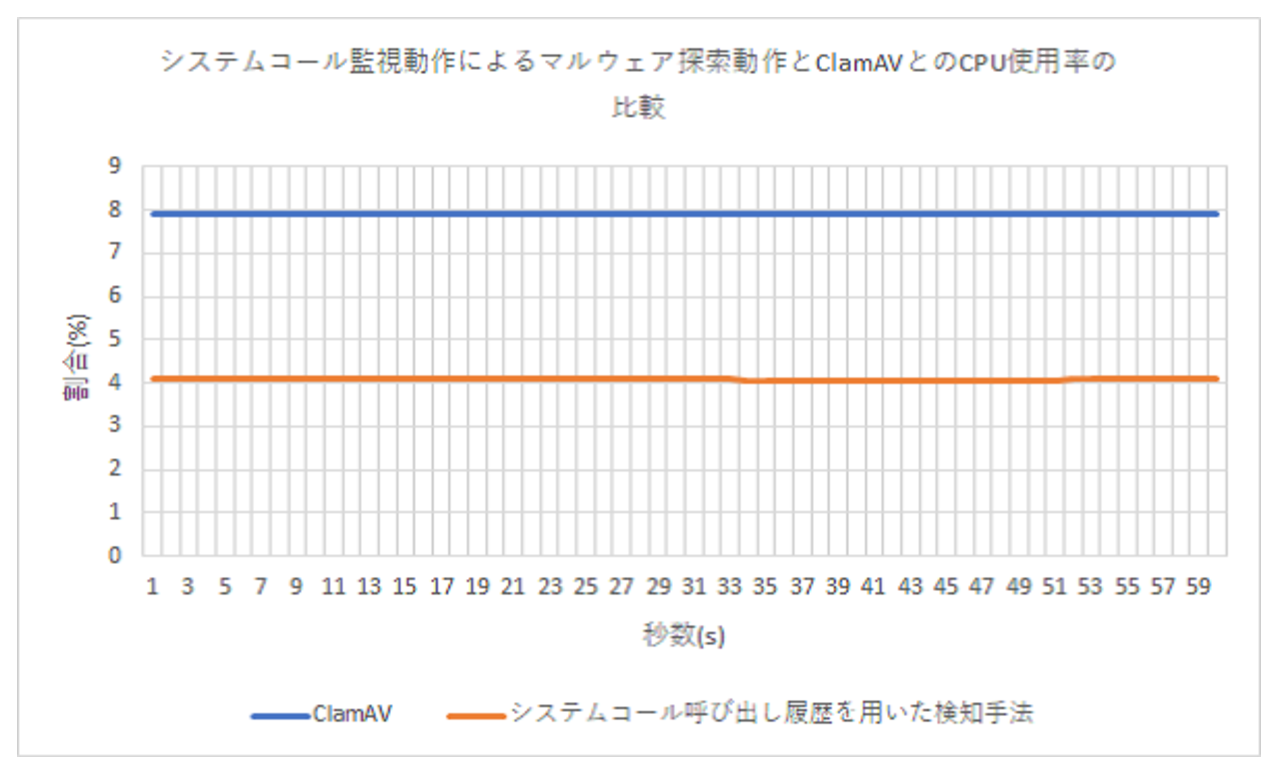
\includegraphics[width=110mm]{figures/strace_mem.eps}
        \caption{IoTデバイス上でマルウェアが動作していない状況におけるマルウェア探索のメモリ使用率}
        \label{fig:strace_mem}
\end{figure}
\newpage
\section{Miraiとその亜種マルウェアを対象とする判別性能評価}
ハニーポットを用いてDDoS攻撃を行うマルウェアを収集し,収集したマルウェアを検体として用いて,システムコール呼び出し履歴を用いた検知手法の検知精度の評価を行い,システムコール呼び出し履歴を用いた検知手法の有効性を確認した.

\subsection{ハニーポットによるマルウェアの収集}
%ハニーポットの説明をもう少し冗長に書いて置く,
ハニーポットと呼ばれる攻撃者に脆弱なシステムであると見せかけることで攻撃者を誘い込み,侵入手法や侵入後に実行されるコマンドのログやダウンロードされるファイルを収集するシステムを用いてDDoS攻撃を行うマルウェアを収集した.ハニーポットのシステムの概要図を図\ref{fig:honey}に示す.シェルの対話の中でダウンロードされるバイナリファイルを実行させることなく保存することが可能なMichel Oosterhofによって開発されたCowrie\cite{Cowrie}と呼ばれるハニーポットを用いた.Cowrieによって収集されたバイナリファイルについてVirus Totalと呼ばれるマルウェア検知オンラインサービスを用いて解析を行い,DDoS攻撃を行うマルウェアの分類を行った.Virus Total\cite{Virus}はユーザーから投稿された検体を54のウィルス対策エンジンによって解析するオンラインサービスであり,投稿された検体についてマルウェアの分類を知ることができる.2019/01/09から2019/01/28の期間でハニーポットを断続的に運用してバイナリファイルの収集を行った.収集したバイナリファイルをVirus Totalに投稿し,Virus Totalの解析結果から,MiraiまたはMiraiの亜種のマルウェアをDDoS攻撃を行うマルウェアとして分類分けした.分析した結果,収集したバイナリファイルは,空ファイルのものや,マルウェアをダウンロードさせ実行させるファイル,DDoS攻撃を行うマルウェアのバイナリファイル等が散見され,DDoS攻撃を行うマルウェアは57検体が存在し,マルウェアの実行可能な検体は49検体であった.実験に使用したマルウェアの検体のハッシュ値を付録に記載する.
%マルウェアの検体についてそれぞれの名称や種類,検知できたのか,できなかった理由の分類,を表にまとめて記載する.
\begin{figure}[h]
    \centering
       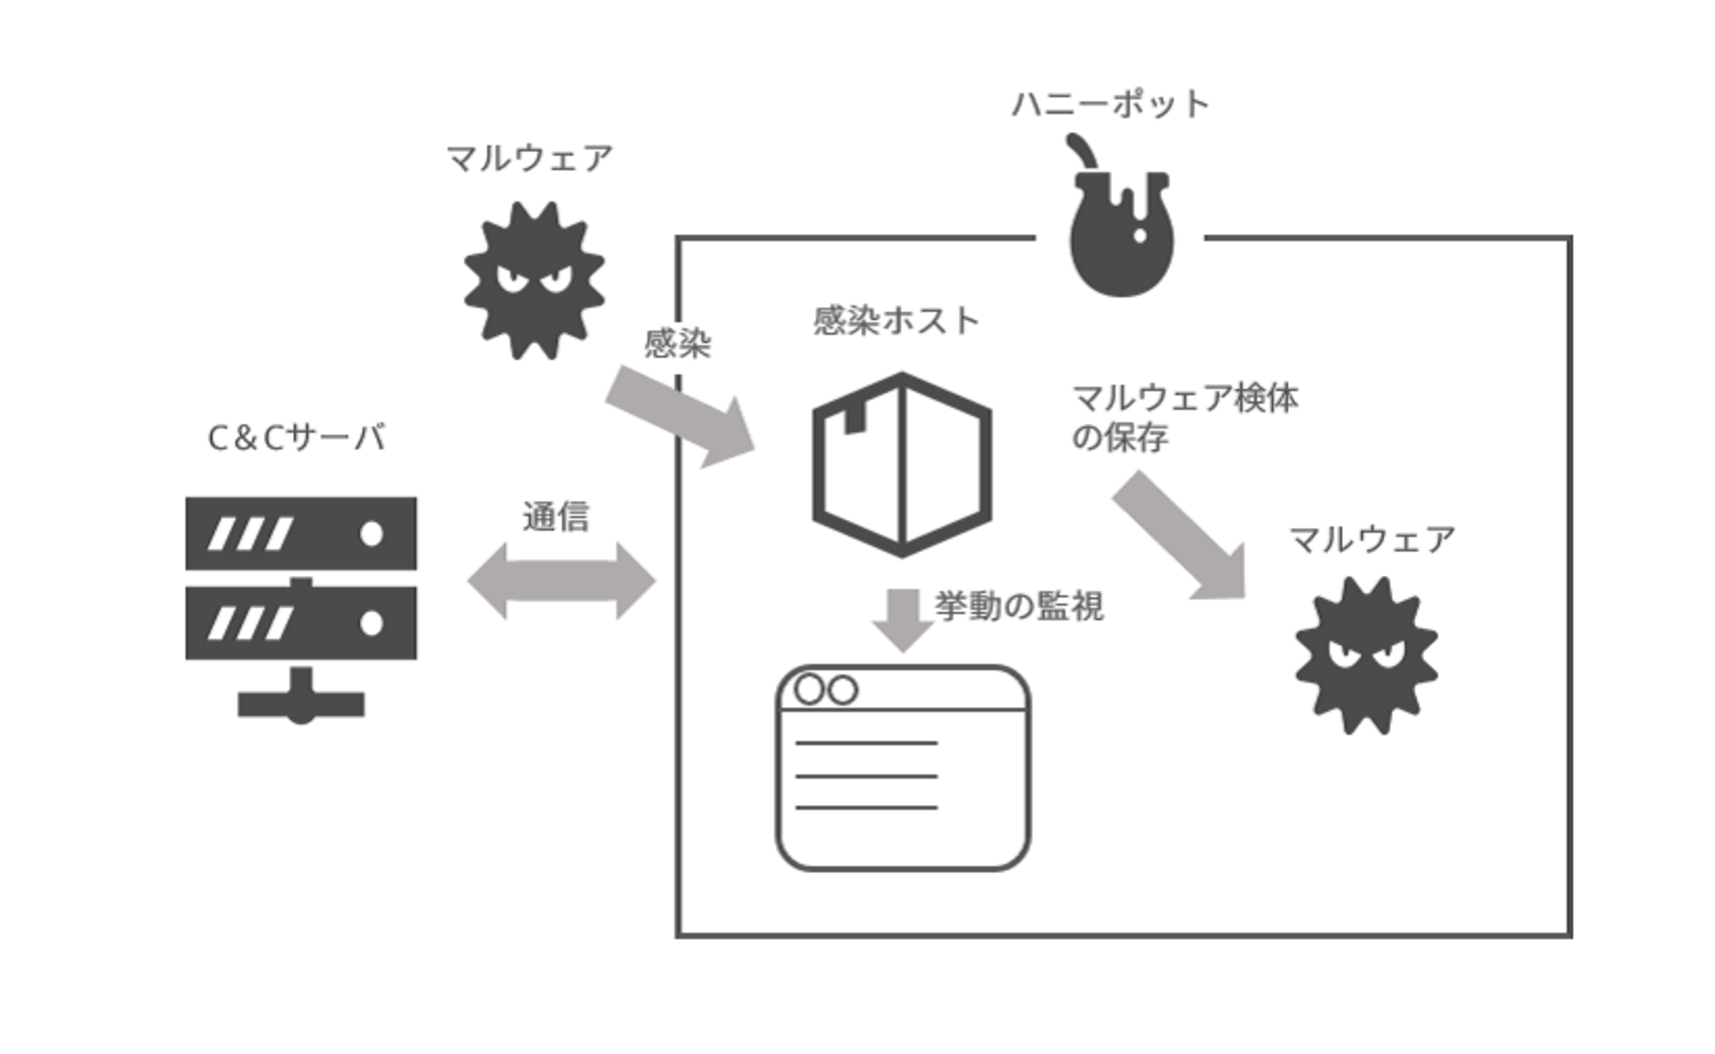
\includegraphics[width=120mm]{figures/honey.eps}
    \caption{ハニーポットのシステム概要図}
    \label{fig:honey}
\end{figure}

\newpage 
\subsection{提案手法によるマルウェアの検知精度評価}
%Linuxのディストリビューションについて明記しておく.
前項で収集したDDoS攻撃を行うマルウェア49検体を用いてシステムコール呼び出し履歴を用いた検知手法の検知精度の評価を行った.入手したマルウェアをネットワークから隔離した状態で検知システムを動作させマルウェアの検出ができるか評価を行った.正規プログラムは,Linuxであるubuntu  16.0 LTS4 LTSに標準でインストールされているプログラムの44検体を利用した.実験の評価指数として,Accuracy,TPR(True Positive Rate),TNR(True Negative Rate),FPR(False Positive Rate),FNR(False Negative Rate)を用いる.Accuracyは,マルウェアを正しく判別できた割合である.TPRはマルウェアをマルウェアと判別できた割合,TNRは正規プログラムを正規プログラムと判別した割合,FNRはマルウェアを正規プログラムと判別した割合,FPRは正規プログラムをマルウェアとして判別した割合である.Accuracy,TPR,TNR,FPR,FNRを下記の式で算出する.

\begin{eqnarray}
    Accuracy & = & \frac{正しくマルウェアと判別された検体数}{検体の総数}\\
    TPR & = & \frac{マルウェア検体がマルウェアと判別された検体数}{マルウェア検体の総数}\\
    TNR & = & \frac{正規プログラムを正規プログラムとして判別された検体数}{正規プログラムの総数}\\
    FNR & = & \frac{マルウェア検体が正規プログラムとして判別された検体数}{マルウェア検体の総数}\\ 
    FPR & = & \frac{正規プログラムをマルウェアとして判別された検体数}{正規プログラムの総数}
\end{eqnarray}
提案システムによるハニーポットで収集したマルウェアの判別結果を表\ref{tab:malware}に示す.プログラムの判別結果を表\ref{tab:detect}に示し,Accuracy,TPR,TNR,FPR,FNRの結果を表\ref{tab:result}に示す.
%提案システムによるプログラムの判別結果を表,\ref{tab:detect}に示し,Accuracy,TPR,TNR,FPR,FNRの結果を表\ref{tab:result}に示す.
\begin{small}
\begin{flushleft}
\begin{longtable}{|c|c|c|c|}
    \caption{49検体のマルウェアの種類と検知の可否}
    \label{tab:malware} \\
    \hline
    検体番号   & マルウェアの種類             & 検知の可否 & 検知できない理由                      \\ \hline
    \endhead
        1  & Linux.Mirai.793      & 可能    & -                             \\ \hline
        2  & Linux.Mirai.793      & 可能    & -                             \\ \hline
        3  & Linux/DDoS-Xor.A     & 可能    & -                             \\ \hline
        4  & Linux/Mirai          & 可能    & -                             \\ \hline
        5  & Linux/Mirai          & 可能    & -                             \\ \hline
        6  & Linux/Mirai          & 可能    & -                             \\ \hline
        7  & Linux/mirai.d        & 可能    & -                             \\ \hline
        8  & Linux/mirai.d        & 可能    & -                             \\ \hline
        9  & Linux/mirai.d        & 可能    & -                             \\ \hline
        10 & Linux/mirai.d        & 可能    & -                             \\ \hline
        11 & Linux/mirai.d        & 可能    & -                             \\ \hline
        12 & Linux/mirai.d        & 可能    & -                             \\ \hline
        13 & Linux/Mirai.f        & 可能    & -                             \\ \hline
        14 & Linux/Mirai.f        & 可能    & -                             \\ \hline
        15 & Linux/Mirai.f        & 可能    & -                             \\ \hline
        16 & Linux/Mirai.f        & 可能    & -                             \\ \hline
        17 & Linux/Mirai.f        & 可能    & -                             \\ \hline
        18 & Linux/Mirai.g        & 可能    & -                             \\ \hline
        19 & Linux/Mirai.g        & 不可    & sendto呼び出しに指定された送信先のポートが52869 \\ \hline
        20 & Linux/Mirai.l        & 可能    & -                             \\ \hline
        21 & Linux/Mirai.l        & 可能    & -                             \\ \hline
        22 & Linux/Mirai.l        & 可能    & -                             \\ \hline
        23 & Linux/Mirai.l        & 可能    & -                             \\ \hline
        24 & Linux/Mirai.l        & 可能    & -                             \\ \hline
        25 & Linux/Mirai.l        & 可能    & -                             \\ \hline
        26 & Linux/Mirai.l       
         & 可能    & -                             \\ \hline
        27 & Linux/Mirai.l        & 不可    & 呼び出されているシステムコールがsendtoではなくsend       \\ \hline
        28 & Linux/Mirai.l        & 不可    & sendto呼び出しに指定された送信先のポートが80    \\ \hline
        29 & RDN/Generic BackDoor & 不可    & スキャン活動を行っていない                 \\ \hline
        30 & RDN/Generic BackDoor & 不可    &   \\ \hline
        31 & RDN/Generic BackDoor & 可能    & -                             \\ \hline
        32 & RDN/Generic BackDoor & 可能    & -                             \\ \hline
        33 & RDN/Generic BackDoor & 可能    & -                             \\ \hline
        34 & RDN/Generic BackDoor & 可能    & -                             \\ \hline
        35 & RDN/Generic BackDoor & 可能    & -                             \\ \hline
        36 & RDN/Generic BackDoor & 不可    & 呼び出されているシステムコールがsendtoではなくsend       \\ \hline
        37 & RDN/Generic BackDoor & 可能    & -                             \\ \hline
        38 & RDN/Generic BackDoor & 可能    & -                             \\ \hline
        39 & RDN/Generic BackDoor & 可能    & -                             \\ \hline
        40 & RDN/Generic BackDoor & 可能    & -                             \\ \hline
        41 & RDN/Generic BackDoor & 可能    & -                             \\ \hline
        42 & RDN/Generic BackDoor & 可能    & -                             \\ \hline
        43 & RDN/Generic BackDoor & 可能    & -                             \\ \hline
        44 & RDN/Generic BackDoor & 可能    & -                             \\ \hline
        45 & RDN/Generic BackDoor & 不可    & sendto呼び出しに指定されたポートが37215      \\ \hline
        46 & RDN/Generic BackDoor & 可能    & -                             \\ \hline
        47 & RDN/Generic BackDoor & 可能    & -                             \\ \hline
        48 & RDN/Generic BackDoor & 可能    & -                             \\ \hline
        49 & RDN/Generic BackDoor & 不可    & 検知プログラムの強制終了                  \\ \hline
    
\end{longtable}
\end{flushleft}
\end{small}

\begin{table}[h]
    \centering
    \caption{提案システムによるマルウェアの判別結果}
    \label{tab:detect}
    \begin{tabular}{cc|c|c|}
    \cline{3-4}
    & \multicolumn{1}{l|}{} & \multicolumn{2}{c|}{判別結果} \\ \cline{3-4} 
    &                       & マルウェア      & 正規プログラム      \\ \hline
    \multicolumn{1}{|c|}{\multirow{2}{*}{真の結果}} & マルウェア                 & 41         & 8            \\ \cline{2-4} 
    \multicolumn{1}{|c|}{}                      & 正規プログラム               & 0          & 44           \\ \hline
    \end{tabular}
    \end{table}

\begin{table}[h]
     \caption{プログラムの判別結果} 
     \label{tab:result}
     \centering 
    \begin{tabular}{|c|c|c|c|c|} \hline 
    Accuracy & TPR    & TNR     & FNR    & FPR   \\ \hline
    91.3\%   & 83.4\% & 100.0\% & 16.6\% & 0.0\% \\ \hline
    \end{tabular}
\end{table}

評価の結果,Accuaryは91.3\%と高い精度となっており,TPRの値が,83.4\%であり,FPRの値が0\%である.TPRが83.4\%のため,Mirai亜種の多くのマルウェアは作成時に元にしたMiraiのスキャン機能をそのまま流用している場合が多いことがわかった.しかし,スキャン活動を行っている一部のマルウェアは提案システムによって検出することができなかった.検出ができなかった要因としてスキャン活動を行っていない場合とスキャン活動を行っている際にスキャンしているポートが23ではなく,他のポートをスキャンしてため,検知条件に一致しなかったためである.TNRが高い精度を示した理由には,対象となっている正規プログラムがubuntu 16.04 LTSに標準でインストールされているプログラムを利用している事が挙げられる.検知条件に一致する組織や個人で作成されたプログラムではsendtoを連続して呼び出すプログラムが存在すると考えられるため誤検知をする可能性がある.

\subsection{考察}
システムコール呼び出し履歴を用いた検知手法とClamAVのメモリ使用率,CPU使用率の比較を行った結果,メモリ使用率が48.4\%減,CPU使用率が97.6\%減となったことから,システムコール呼び出し履歴を用いた検知手法はIoTデバイスの本来の動作を阻害することがなくIoTデバイスがマルウェアに感染していないことを確認する事ができる.Accuaryは91.3\%と高い精度となっており,DDoS攻撃を行うマルウェアを検出するのに有効である.したがって,マルウェアの内部関数によって呼び出されるシステムコール系列をもとにマルウェアを検出することによって,IoTデバイスなどの計算資源の乏しい端末でもホスト上でのマルウェアに対して有効なセキュリティ対策が行えると考えられる.